% !TEX root = ../keldysh_main.tex
\sloppy
%\pagenumbering{arabic} \setcounter{page}{1}
\thispagestyle{empty}

%%%%%%%%%%%%%%%%%%%%%%%%%%%%%%%%%%%%%%%%%%%%%%%%%%%%%%%%%%%%%

%Обязательно заполните следующие поля - для оглавления и колонтитулов!!!:


\addtocontents{toc}{\protect\vspace{4pt}}
\addtocontents{toc}{\noindent\textbf{Беспятый Илья Витальевич} \quad \emph{МГУ имени М.В.Ломоносова (Россия, Москва)}
\\} %Please, don't change the height of the letters!

\addtocontents{toc}{\protect\vspace{-9.5pt}}
\addcontentsline{toc}{art}{\qquad\textsc {Разработка и исследование прототипа абсолютного датчика угла для астрономического телескопа}} %Пожалуйста, не меняйте высоту букв! Название должно совпадать с названием Вашей курсовой (или выпускной) работы.

%   6 обязательных для заполнения пунктов:
\noindent {\footnotesize УДК: 681.785.5}

\title{РАЗРАБОТКА И ИССЛЕДОВАНИЕ ПРОТОТИПА АБСОЛЮТНОГО ДАТЧИКА УГЛА ДЛЯ АСТРОНОМИЧЕСКОГО ТЕЛЕСКОПА. } %Пожалуйста, не меняйте высоту букв!
\markboth{Разработка и исследование прототипа абсолютного датчика угла для астрономического телескопа}{Разработка и исследование прототипа абсолютного датчика угла для астрономического телескопа}%Это название будет печататься в колонтитулах. Если полное название слишком большое, запишите здесь краткое название статьи.

\author{Беспятый И.\;В.} %Пожалуйста, не меняйте высоту букв!

\address{МГУ имени М.В. Ломоносова (Россия, Москва)}

\email{ilia@bespyatyy.ru}

\begin{abstract}
В данной работе разработан и исследован прототип абсолютного оптического датчика угла для астрономического телескопа АЗТ-6 КГО ГАИШ МГУ. Рассмотрены источники погрешностей угловых энкодеров; обоснован выбор однодорожечной кодовой структуры на основе псевдослучайной последовательности де~Брейна и метода путевого усреднения двух диаметрально расположенных считывающих головок для подавления систематических ошибок.

Разработана и реализована полная цепочка алгоритмической обработки сигнала ПЗС-матрицы: калибровка радиальной дисторсии линзы по образу периодической «зебры», субпиксельное обнаружение фронтов методом Блэ--Риу, восстановление битовой последовательности и оценка абсолютного угла методом взвешенного кругового среднего по скользящему окну. Алгоритм верифицирован на синтетической модели: при отношении сигнал/шум не менее $10$~дБ достигнуто СКО определения фронтов менее 0.1~пикс и стопроцентная точность восстановления последовательности.

Экспериментально подтверждена эффективность метода путевого усреднения: СКО угловой погрешности снизилось с $0.08^\circ$ до $0.06^\circ$ при максимальном отклонении не более $0.08^\circ$. Ограничивающим фактором точности прототипа является точность нанесения растра методом 3D-печати; для дальнейшего улучшения предложено применение фотолитографически изготовленного диска.

Программный код проекта доступен по ссылке: \url{https://github.com/shroomjak/EncoderDecoder.git}.\\
\emph{Ключевые слова:} {абсолютный энкодер, оптический датчик угла, последовательность де~Брейна, субпиксельная обработка, метод Блэ--Риу, коррекция дисторсии, астрономическая монтировка}
\end{abstract}



\bigskip

% для статьей на русском обязателен перевод 4 пунктов (кроме УДК и электронной почты) на английский:

\title{\uppercase{DEVELOPMENT AND INVESTIGATION OF AN ABSOLUTE ANGLE ENCODER PROTOTYPE FOR AN ASTRONOMICAL TELESCOPE. }} %Пожалуйста, не меняйте высоту букв! Перевод должен совпадать с переводом названия Вашей курсовой (или выпускной) работы.

\author{Bespyatyy Ilia} %Пожалуйста, не меняйте высоту букв!

\address{Moscow Lomonosov State University}

\begin{abstract}

In this work, a prototype of an absolute optical angle sensor for the AZT-6 telescope at the Caucasian Mountain Observatory of SAI MSU is developed and investigated. The sources of angular encoder errors are analyzed; the choice of a single-track code structure based on a De~Bruijn pseudorandom sequence and the two-head averaging method with diametrically opposed read heads for suppression of systematic errors is justified.

A complete signal processing pipeline for the CCD line sensor is developed and implemented: calibration of the lens radial distortion using a periodic zebra pattern, sub-pixel edge detection via the Blais--Rioux filter, bit sequence reconstruction, and absolute angle estimation by weighted circular mean over a sliding window. The algorithm is validated on a synthetic model: at SNR $\geq 10$~dB, edge position RMS below 0.1~pixel and 100\% bit sequence reconstruction accuracy are achieved.

The effectiveness of the two-head averaging method is confirmed experimentally: the RMS angular error decreased from $0.08^\circ$ to $0.06^\circ$, with a maximum deviation not exceeding $0.08^\circ$. The limiting factor of the prototype accuracy is the precision of the grating produced by 3D printing; application of a photolithographically manufactured disk is proposed for further improvement.

Source code: \url{https://github.com/shroomjak/EncoderDecoder.git}.\\
\emph{Keywords:} {absolute encoder, optical angle sensor, De~Bruijn sequence, sub-pixel processing, Blais--Rioux filter, distortion correction, astronomical mount}
\end{abstract}


%\bigskip
\section{Введение}

Проведение современных астрономических наблюдений предполагает высокую точность наведения и сопровождения телескопов: ошибки в определении углового положения элементов системы приводят к смещению изображения небесного объекта и снижению качества получаемых данных. Среди датчиков углового положения наибольшее распространение получили \emph{абсолютные энкодеры}, обеспечивающие однозначное определение углового положения без необходимости повторной инициализации.

Актуальность задачи обусловлена постоянным ростом требований к точности астрономических установок. Современные телескопы требуют измерения углов с погрешностью от единиц до десятых долей угловых секунд при устойчивости к вибрациям, температурным колебаниям и загрязнению. При этом промышленные решения для робототехники и станков часто не удовлетворяют требованиям астрономии, а специализированные энкодеры ведущих производителей (Heidenhain, Renishaw, Celera Motion) имеют высокую стоимость.

Дополнительную сложность вносит конструктивная особенность телескопов: их оси не могут совершать полного оборота в рабочем режиме, что исключает прямое применение классических алгоритмов самокалибровки (EDA, метод Масуды, VEDA), рассчитанных на многооборотный режим. Снижение погрешности энкодера в таких условиях должно достигаться  методами и алгоритмами обработки сигнала, применимыми в ограниченном рабочем диапазоне оси.

\textbf{Цель работы} --- разработка и исследование прототипа абсолютного датчика угла для астрономического телескопа на основе оптического принципа измерения.

\textbf{Задачи работы:}
\begin{itemize}
    \item провести анализ существующих технологий и конструкций абсолютных энкодеров, применяемых в высокоточных системах;
    \item определить ключевые метрологические и эксплуатационные требования к датчику угла для астрономических установок;
    \item разработать концепцию и изготовить прототип абсолютного энкодера;
    \item провести экспериментальные исследования полученного образца и оценить его характеристики.
\end{itemize}

Объектом применения разрабатываемого прототипа выбран астрономический рефлектор АЗТ-6 КГО ГАИШ МГУ с немецкой экваториальной монтировкой.

\section{Постановка проблем и инструменты их решения}

\subsection{Источники погрешностей оптического энкодера}

Полная погрешность оптического углового энкодера формируется из нескольких основных составляющих: ошибки нанесения шкалы, эксцентриситета шкалы (смещение геометрического центра растра относительно оси вращения), деформаций формы шкалы (высшие гармоники) и ошибок считывающей головки. 

Суммарная ошибка после установки энкодера (ошибка установки) включает ошибку системы <<шкала-головка>>, основные слагаемые которой описаны выше, а также дополнительные составляющие, внесенные условиями монтажа, например, люфты и дребезги креплений, подшипников и т.д. Именно эта величина является практически значимой характеристикой для конкретного применения.

\subsection{Модель наведения}

При анализе точности измерений на астрономических телескопах необходимо учитывать, что погрешность углового датчика входит в общую ошибку наведения монтировки и тем самым влияет на качество построения её параметрической модели. Для описания и идентификации систематических ошибок наведения в астрономической практике применяется пакет \textit{TPOINT}~\cite{TPoint_Wallace}, в рамках которого отклонения измеренного положения объекта от расчётного представляются через набор стандартных коэффициентов модели. К числу таких коэффициентов относятся, в частности, поправки нулевых положений по двум осям, а также параметры, характеризующие неперпендикулярность осей и ошибки полярной установки. В связи с этим любая ошибка показаний энкодера приводит к увеличению остатков при идентификации модели и ухудшает точность наведения телескопа в рабочей области. Поэтому задачу повышения точности энкодера следует рассматривать не изолированно, а как часть общей задачи повышения точности измерений и наведения астрономической установки.

\subsection{Постановка задачи самокоррекции и самокалибровки в условиях ограниченного хода оси}

Ключевая практическая проблема работы: астрономический телескоп с немецкой экваториальной монтировкой \emph{не может совершать полный оборот} по полярной оси. Это исключает прямое применение классических алгоритмов самокоррекции (EDA, метод Масуды, VEDA), рассчитанных на полно и/или многооборотный режим. Снижение погрешности энкодера должно достигаться конструктивными методами и алгоритмами обработки сигнала, применимыми в рабочем диапазоне оси.

Суммарная погрешность энкодера $\sigma_{\mathrm{enc}}$ непосредственно определяет ширину буферов безопасности вокруг запретных зон (меридианная зона, упоры монтировки), вынуждая увеличивать «мертвые» угловые диапазоны. Снижение $\sigma_{\mathrm{enc}}$ напрямую расширяет рабочее поле инструмента.

\subsection{Метод путевого усреднения двух диаметрально расположенных головок}

В качестве основного конструктивного решения по снижению систематической погрешности выбран \emph{метод путевого усреднения (МПУ)} с двумя диаметрально противоположными считывающими головками~\cite{mpu-ionak,mpu-bachish,heidenhain-modular-angle-encoders}. При $N=2$ из суммарного сигнала исчезают все нечетные гармоники погрешности, включая доминирующую первую (эксцентриситет):
\begin{equation*}
    \bar{\theta} = \frac{1}{2}\bigl(\theta_1(\varphi) + \theta_2(\varphi + \pi)\bigr).
\end{equation*}

\subsection{Кодовая структура растра и ограничения прототипа}

Кодовая дорожка диска представляет собой псевдослучайную последовательность де~Брейна: любое окно из $n$ последовательных бит уникально и однозначно определяет угловое положение. Для прототипа изготовленного методом 3D-печати, в результате экспериментов и измерений были установлены следующие параметры:

\begin{table}[ht!]
    \centering
    \begin{tabular}{l|c|c}
        \hline
        Параметр & Ограничение & Значение \\
        \hline
        Ширина бита растра $w$, мм & $\geq 0.5$ & $1.6$ \\
        Масштаб проецирования $\lambda$, пикс/мм & $\geq 3$ & $3.75$ \\
        Ширина бита в пикселях $k$, пикс & $\geq 3$ & $6$ \\
        Длина поля зрения $L$, мм & $\leq 30$ & $24$ \\
        Радиус дорожки $R$, мм & $\leq 100$ & $100$ \\
        Длина кодового слова $n$, бит & --- & $9$ \\
        \hline
    \end{tabular}
    \caption{Параметры конструкции прототипа}
\end{table}

Оцененное СКО определения углового положения телескопа по используемому алгоритму составило $\sigma(k) \leq 0.1$ пикс., таким образом оценка сверху на угловое разрешение одиночного измерения составляет:
\begin{equation*}
    \rho = \frac{\sigma}{R \cdot \lambda} \simeq 55''.
\end{equation*}

\subsection{Задача коррекции дисторсии линзы}

Для обеспечения достаточного числа пикселей на бит растра в считывающей головке используется линза, которая вносит радиальную дисторсию. Применяется модель деления~\cite{aleman_lens_distortion}:
\begin{equation*}
    x_d = \frac{x_u}{1 + k\,x_u^2},
\end{equation*}
где $x_u$ --- неискаженная, $x_d$ --- наблюдаемая нормированная координата. Задача: по сигналу с равномерного калибровочного растра («зебры») оценить коэффициент $k^*$ и скорректировать сигнал перед восстановлением битовой последовательности.

\section{Ход выполнения работы}

\subsection{Прототип и установка}

Прототип энкодера разработан для телескопа АЗТ-6 КГО ГАИШ МГУ Кодовый диск изготовлен методом 3D-печати, считывающие головки содержат линзу и линейную ПЗС-матрицу. Две головки расположены диаметрально противоположно для подавления ошибки эксцентриситета.

\begin{figure}[ht!]
    \centering
    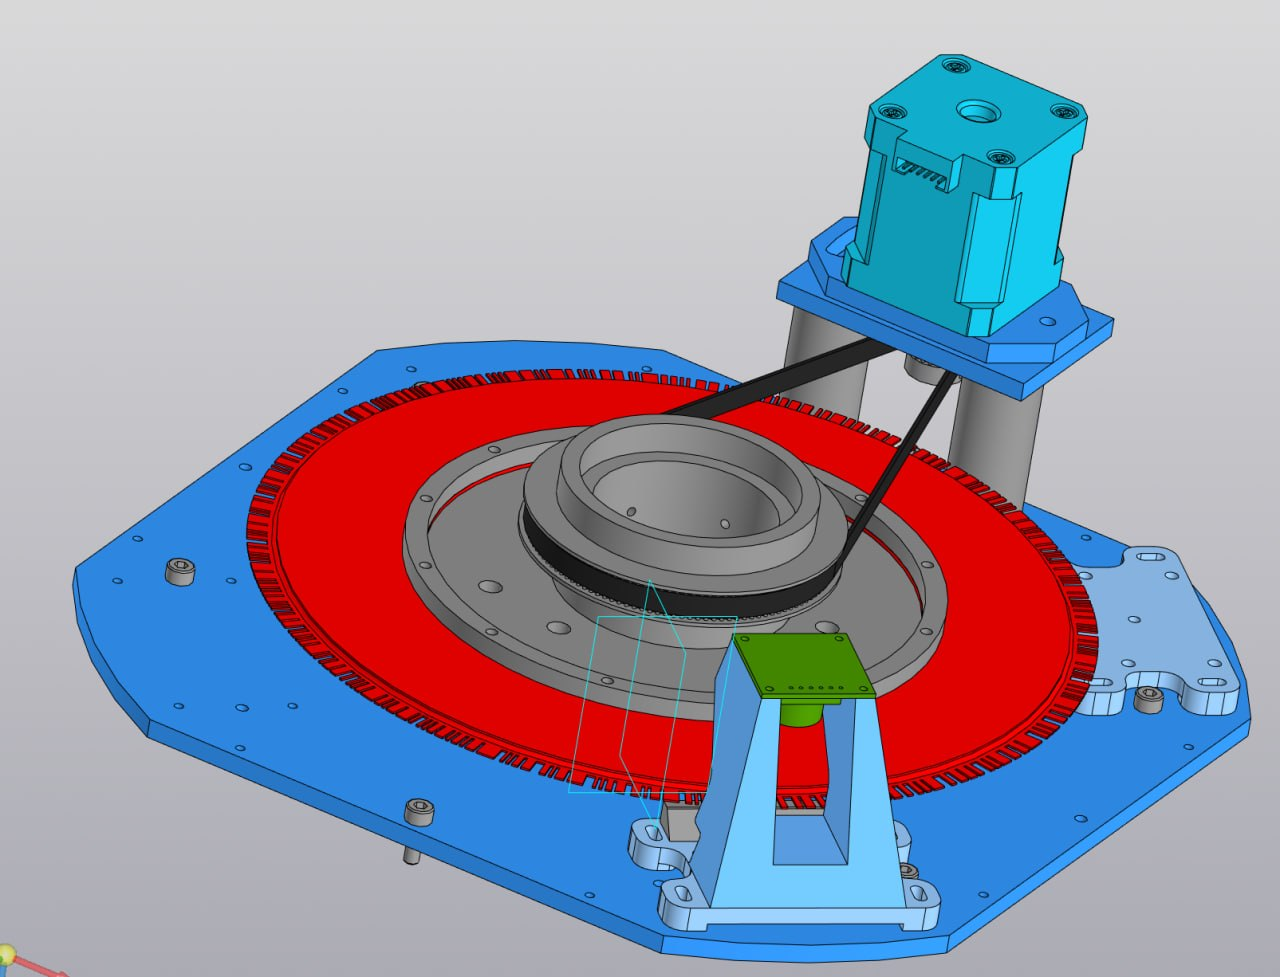
\includegraphics[width=0.75\linewidth]{BespyatyyIV/images/3D модель.png}
    \caption{3D"=модель узла энкодера на АЗТ-6}
    \label{fig:3d_model}
\end{figure}

\subsection{Калибровка дисторсии линзы}

На ПЗС-матрицу проецируется образ периодической «зебры» (см. Приложение, рис. \ref{zebra}). По субпиксельным координатам одноименных фронтов (только восходящих или только нисходящих) минимизируется дисперсия межфронтовых расстояний по $k$. Устойчивое обратное преобразование:
\begin{equation*}
    x_u = \frac{2x_d}{1 + \sqrt{1 - 4k\,x_d^2}}.
\end{equation*}
По серии из трех измерений получены: $k_1^* \simeq 0.052$ (первая головка), $k_2^* \simeq 0.050$ (вторая головка).

\subsection{Алгоритм обработки сигнала и восстановления битовой последовательности}

Полная цепочка обработки сигнала ПЗС"=матрицы:
\begin{enumerate}
    \item \textbf{Геометрическая коррекция дисторсии} по калиброванному $k^*$ с интерполяцией на равномерную сетку.
    \item \textbf{Нормализация, гауссово сглаживание, коррекция виньетирования}: сигнал приводится к единичному диапазону, применяется сглаживание с параметром $\sigma$, затем делится на измеренный профиль виньетирования для каждой головки отдельно.
    \item \textbf{Дифференциальный фильтр Блэ--Риу} ($N=2$)~\cite{blais_rioux_peak}: вычисляются сглаженные первая и вторая производные. Ядро фильтра:
        \begin{equation*}
            \mathrm{BR} = \frac{1}{2N}\bigl[\underbrace{-1,\ldots,-1}_{N},\;0,\;\underbrace{1,\ldots,1}_{N}\bigr].
        \end{equation*}
    \item \textbf{Субпиксельное обнаружение фронтов} по нулям второй производной с линейной интерполяцией, пороговая фильтрация по амплитуде $|D_1|$ и минимальному расстоянию между фронтами.
    \item \textbf{Восстановление битовой последовательности}: число битов в сегменте $n_i = \mathrm{round}((p_{i+1}-p_i)/k)$, значение бита --- знак $D_1$ в левом фронте.
\end{enumerate}

На синтетическом сигнале при SNR $\geq 10$~дБ достигнуто: СКО положений фронтов менее 0.1~пикс ($< 2\%$ ширины бита), точность восстановления последовательности --- 100\%.

\subsection{Оценка абсолютного угла}

По восстановленной последовательности строится скользящее окно длиной $n$ бит. Каждое кодовое слово ищется в кодовой таблице соответствий. Итоговая оценка угла --- взвешенное круговое среднее по всем окнам поля зрения с весами по профилю виньетирования:
\begin{equation*}
    \bar\theta = \mathrm{arg}\!\left(\sum_j w_j \, e^{\,i\,\theta_j}\right).
\end{equation*}
Выбросы исключаются итерационной процедурой по круговому СКО. Внешний вид рабочего прототипа и пример вывода рабочей программы приведен на рис. \ref{fig:setup_photo}, \ref{fig:phys_model}.
\begin{figure}[ht!]
    \centering
    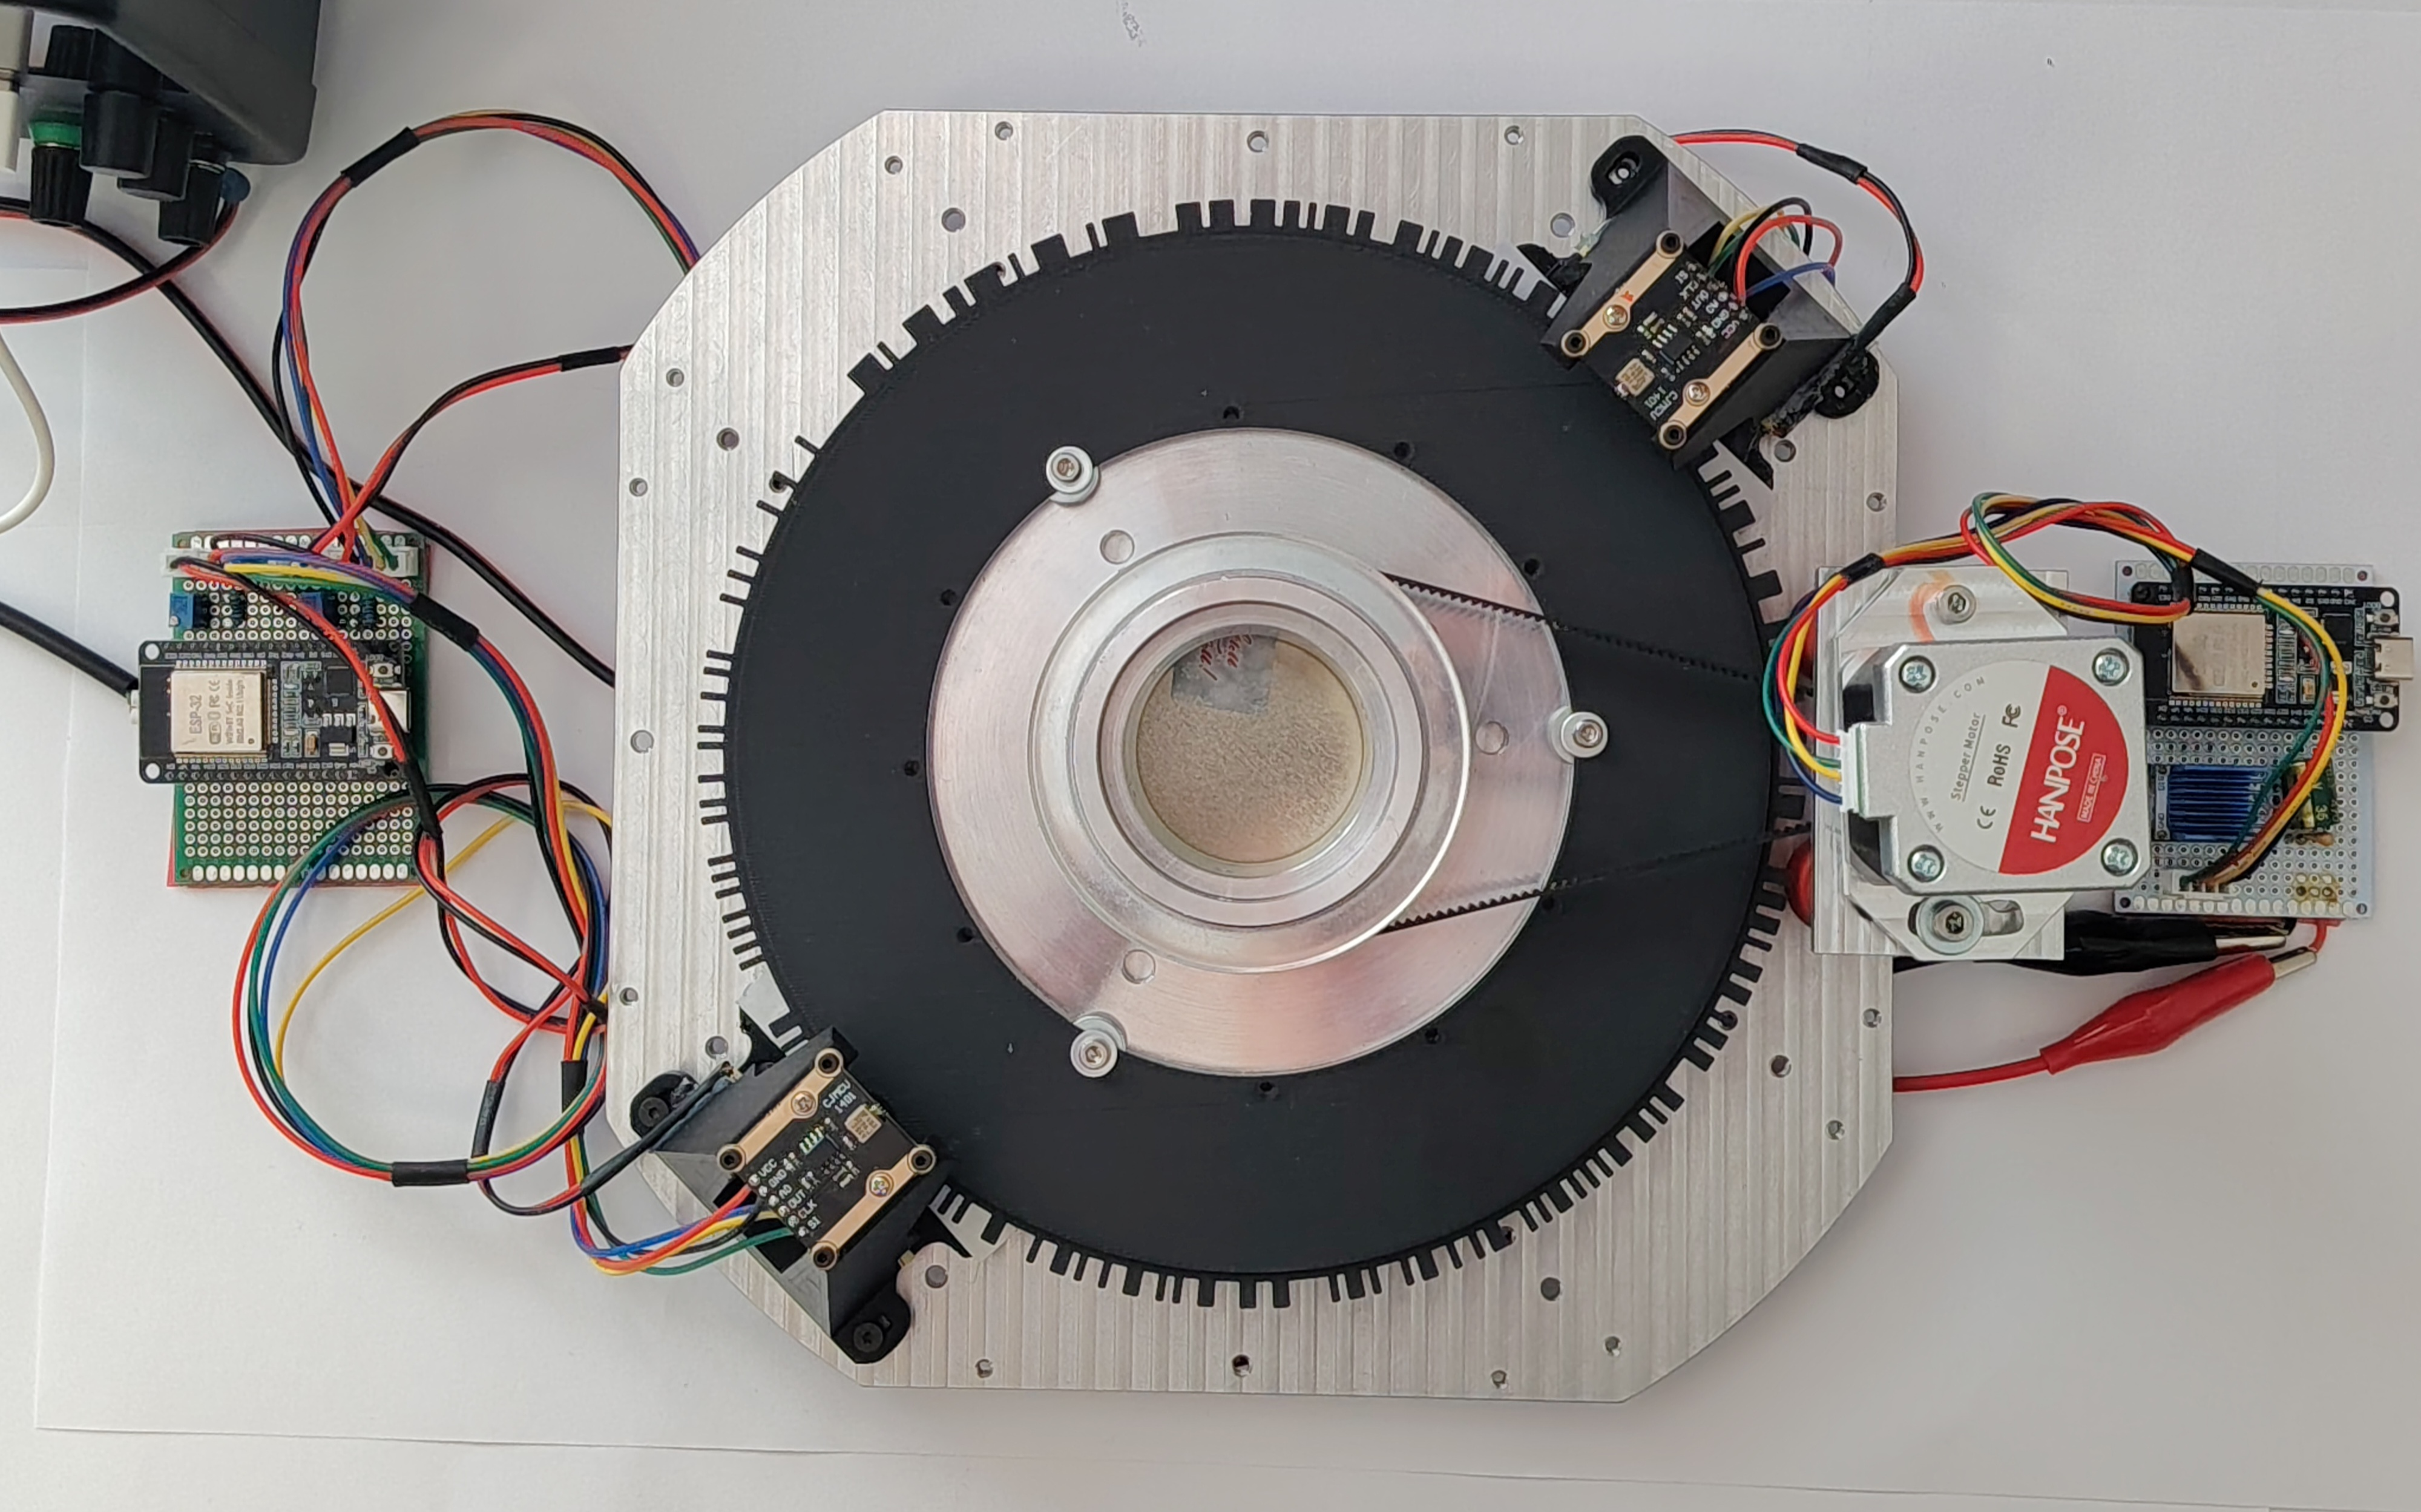
\includegraphics[width=0.95\linewidth]{BespyatyyIV/images/установка две головки.jpg}
    \caption{Фото экспериментальной установки с двумя считывающими головками и кодовым диском}
    \label{fig:setup_photo}
\end{figure}
\newpage
\begin{figure}[ht!]
    \centering
    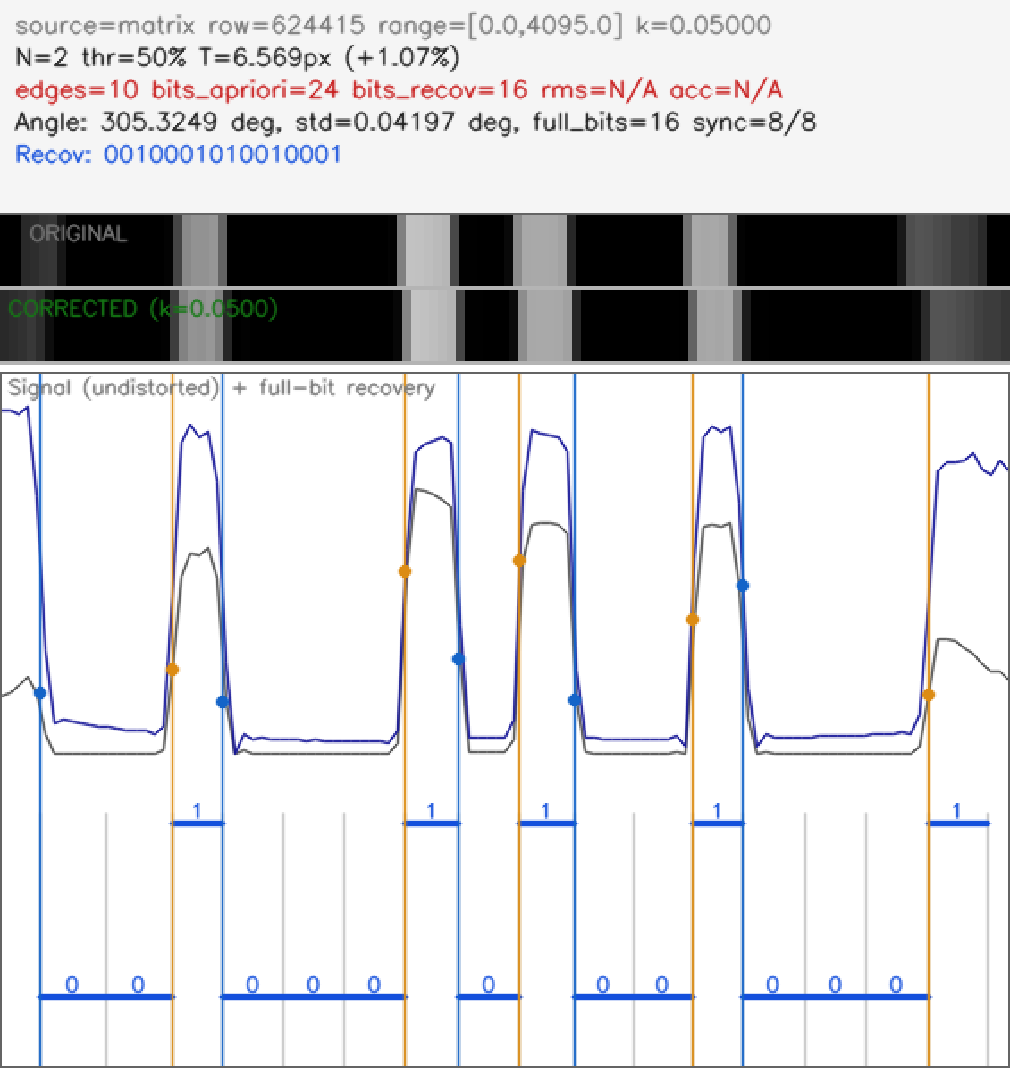
\includegraphics[width=\linewidth]{BespyatyyIV/images/Blais-Rioux Edge Detector.png}
    \caption{Результат работы алгоритма на реальном сигнале с ПЗС"=матрицы}
    \label{fig:phys_model}
\end{figure}
\section{Анализ результатов. Экспериментальная оценка точности}

Для оценки точности энкодера проведена серия измерений при равномерном вращении кодового диска шаговым двигателем по и против часовой стрелки. Эксперименты выполнены как для каждой из двух диаметрально противоположных считывающих головок по отдельности, так и для их кругового среднего. Предварительно для каждой головки независимо выполнена калибровка: измерены плоские поля виньетирования, оценены коэффициенты дисторсии, определено эффективное фокусное расстояние.

\textbf{Основные результаты:}
\begin{itemize}
    \item Установлена зависимость СКО от направления вращения: при вращении, совпадающем с направлением считывания матрицы, СКО ниже, чем при противоположном направлении.
    \item Усреднение показаний двух головок методом кругового среднего подавляет периодическую систематическую погрешность: первая гармоника практически исчезает, наиболее выраженной в остатке остается вторая.
    \item Уровень СКО при усреднении снизился с $\sim 0.08^\circ$ (одна головка, см. Приложение рис. \ref{fig:head1}, \ref{fig:head2}) до $\sim 0.06^\circ$ (круговое среднее, см. Приложение рис. \ref{fig:avg}), что соответствует уменьшению в $\approx\sqrt{2}$ раз при некоррелированных ошибках головок:
        \begin{equation*}
            \sigma_{\mathrm{avg}} = \frac{1}{2}\sqrt{\sigma_1^2 + \sigma_2^2}.
        \end{equation*}
    \item Максимальное отклонение измеряемого угла при усреднении двух головок составило не более $0.08^\circ$ при вращении против считывания; воспроизводимость при вращении в обе стороны --- $0.1^\circ$.
\end{itemize}

\section{Заключение}

В ходе выполнения курсовой работы была решена актуальная задача разработки и исследования прототипа абсолютного оптического датчика угла для астрономического телескопа АЗТ-6 КГО ГАИШ МГУ.

\textbf{Основные результаты и выводы:}
\begin{enumerate}
    \item Проведен анализ существующих технологий абсолютных угловых энкодеров и методов их калибровки; обоснован выбор оптического принципа считывания с однодорожечной кодовой структурой на основе последовательности де~Брейна.

    \item Разработаны и реализованы алгоритмы: калибровки дисторсии линзы по образу периодической «зебры», субпиксельного обнаружения фронтов методом Блэ--Риу, восстановления битовой последовательности и оценки абсолютного угла по скользящему окну с весовой функцией виньетирования.

    \item Изготовлен и экспериментально исследован макет энкодера с двумя диаметрально расположенными считывающими головками (кодовый диск $D=200$~мм, 3D"=печать). Метод путевого усреднения двух головок подтвержден экспериментально: подавлена первая гармоника систематической погрешности, СКО снизилось с $\sim 0.08^\circ$ до $\sim 0.06^\circ$.

    \item Достигнутые метрологические характеристики прототипа: угловое разрешение $\sim 55''$, максимальное отклонение $\leq 0.08^\circ$, воспроизводимость $\sim 0.1^\circ$. Ограничивающим фактором является точность изготовления растра методом 3D"=печати.

    \item Показано, что дальнейшее повышение точности возможно за счет применения фотолитографически изготовленного растра и увеличения числа считывающих головок.
\end{enumerate}

\section*{Приложение}
\addcontentsline{toc}{section}{Приложение}

\begin{figure}[ht!]
    \centering
    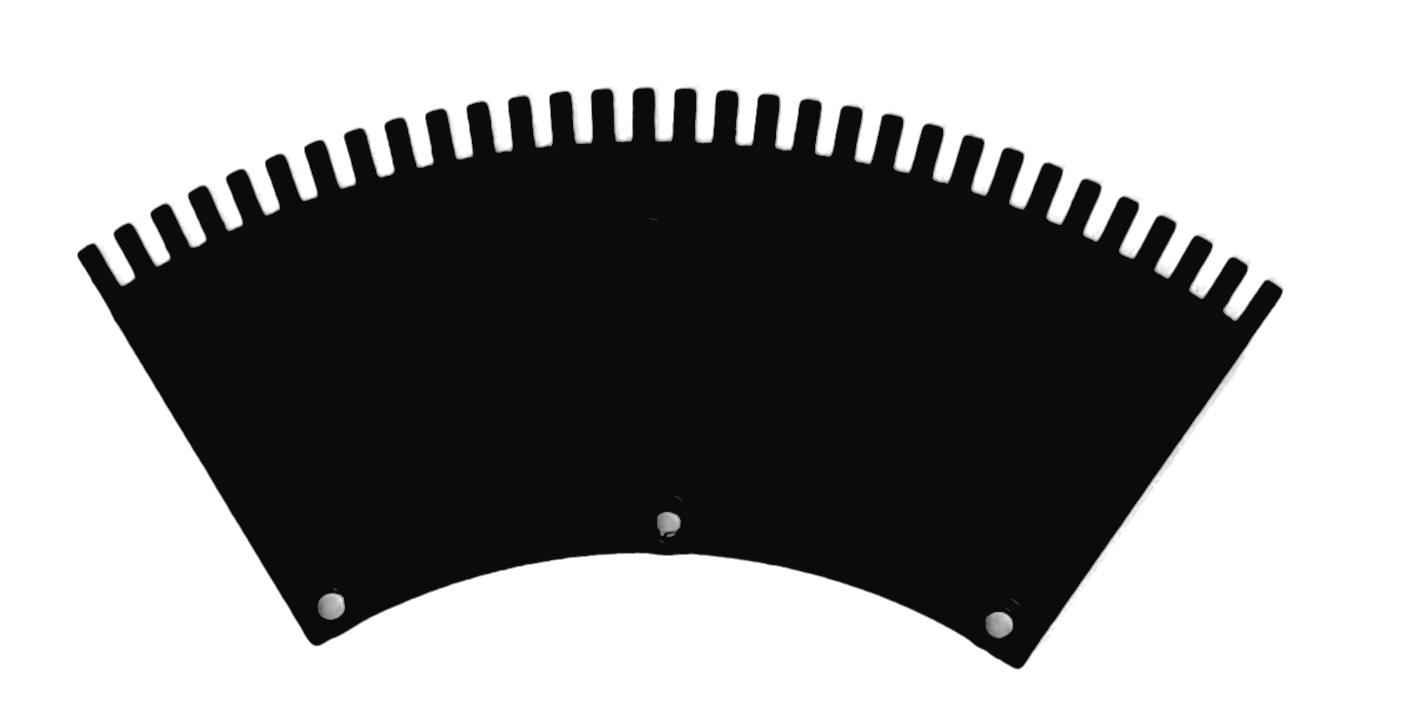
\includegraphics[width=0.5\linewidth]{BespyatyyIV/images/Зебра.jpg}
    \caption{Калибровочная «зебра»}
    \label{zebra}
\end{figure}
\newpage
\begin{figure}[ht!]
    \centering
    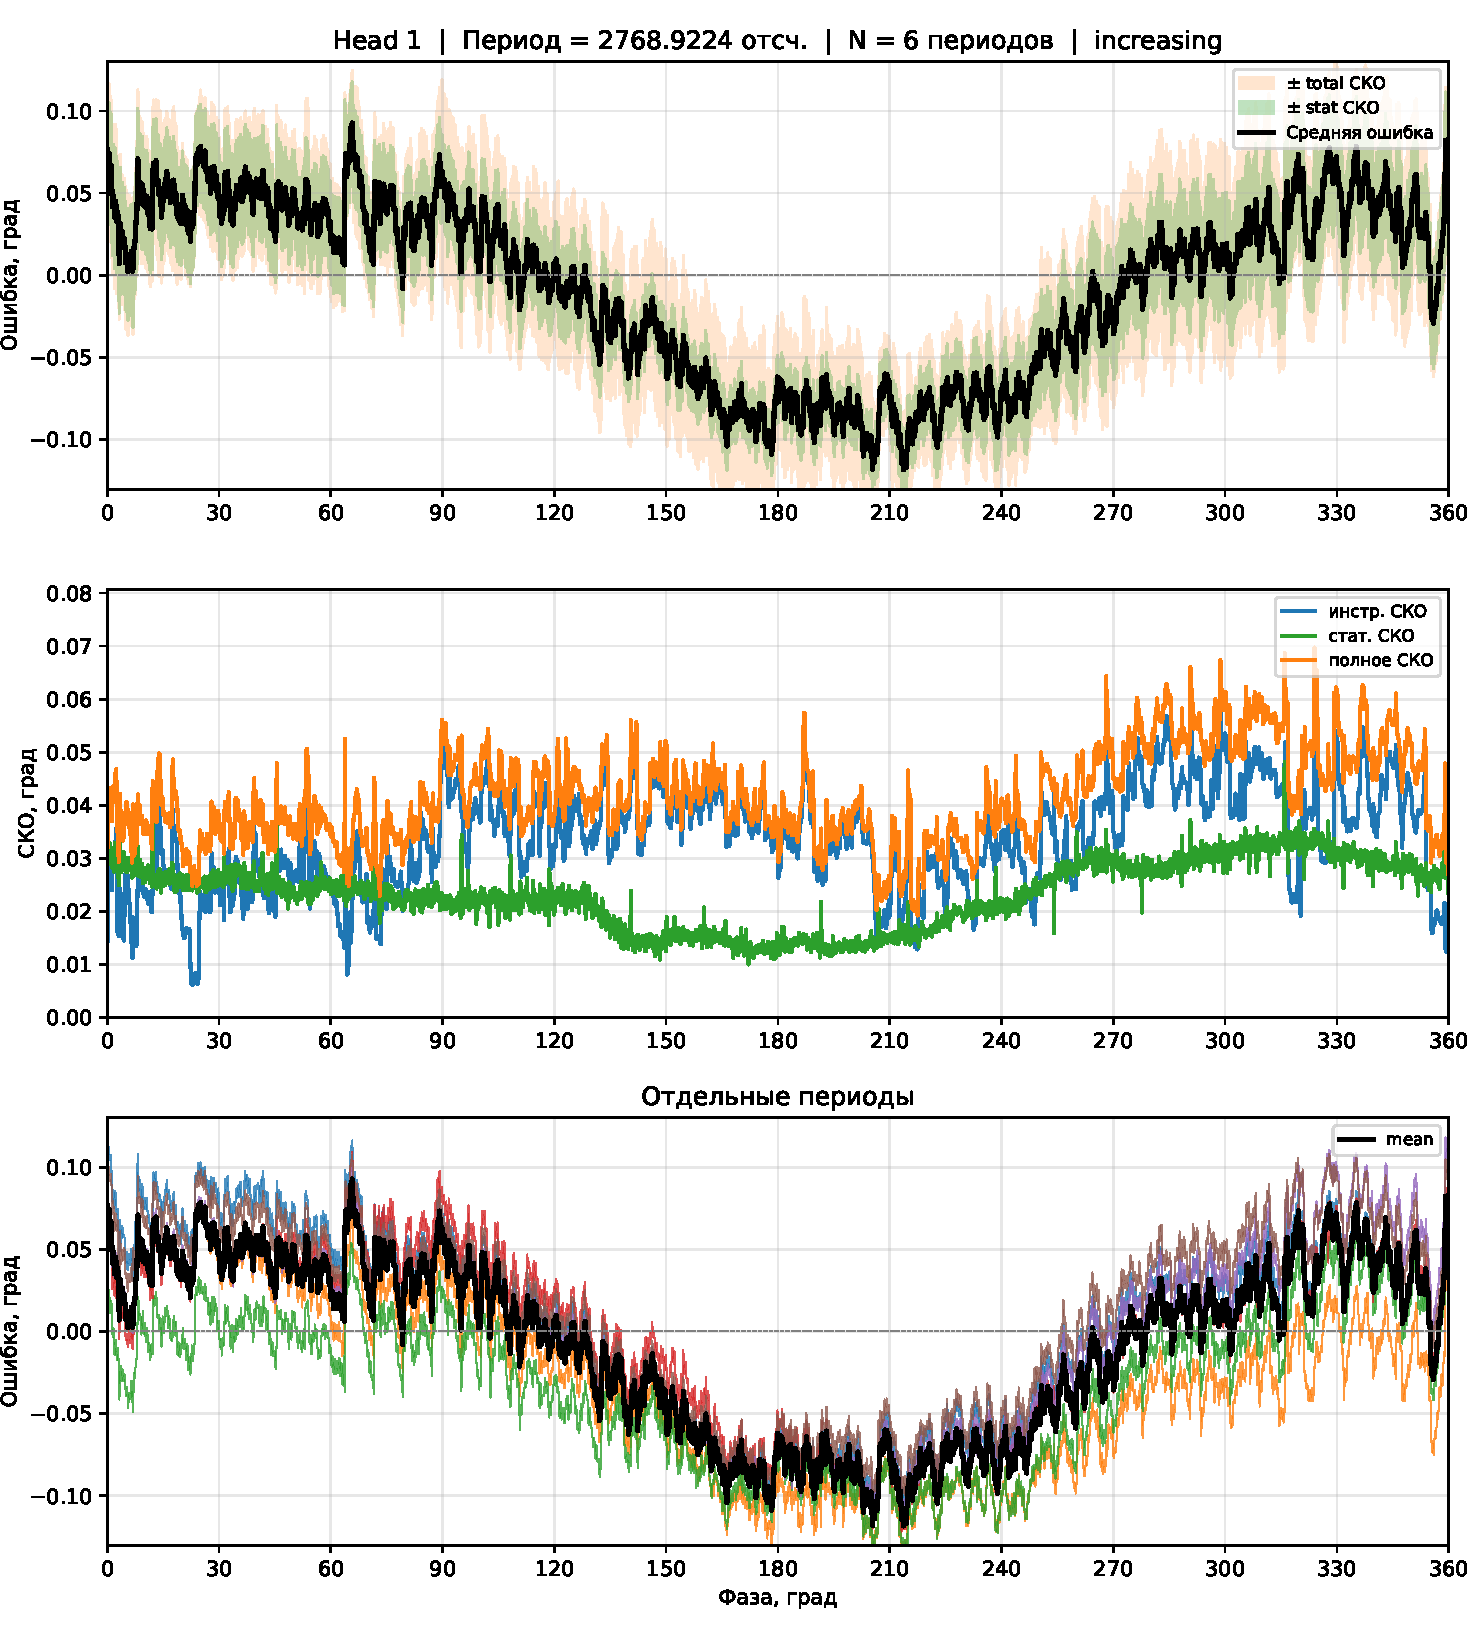
\includegraphics[width=\linewidth]{BespyatyyIV/images/final_10_5000_head1.pdf}
    \caption{Детрендированное усредненное по периодам показание первой головки при скорости 5000~микрошагов/с}
    \label{fig:head1}
\end{figure}
\newpage
\begin{figure}[ht!]
    \centering
    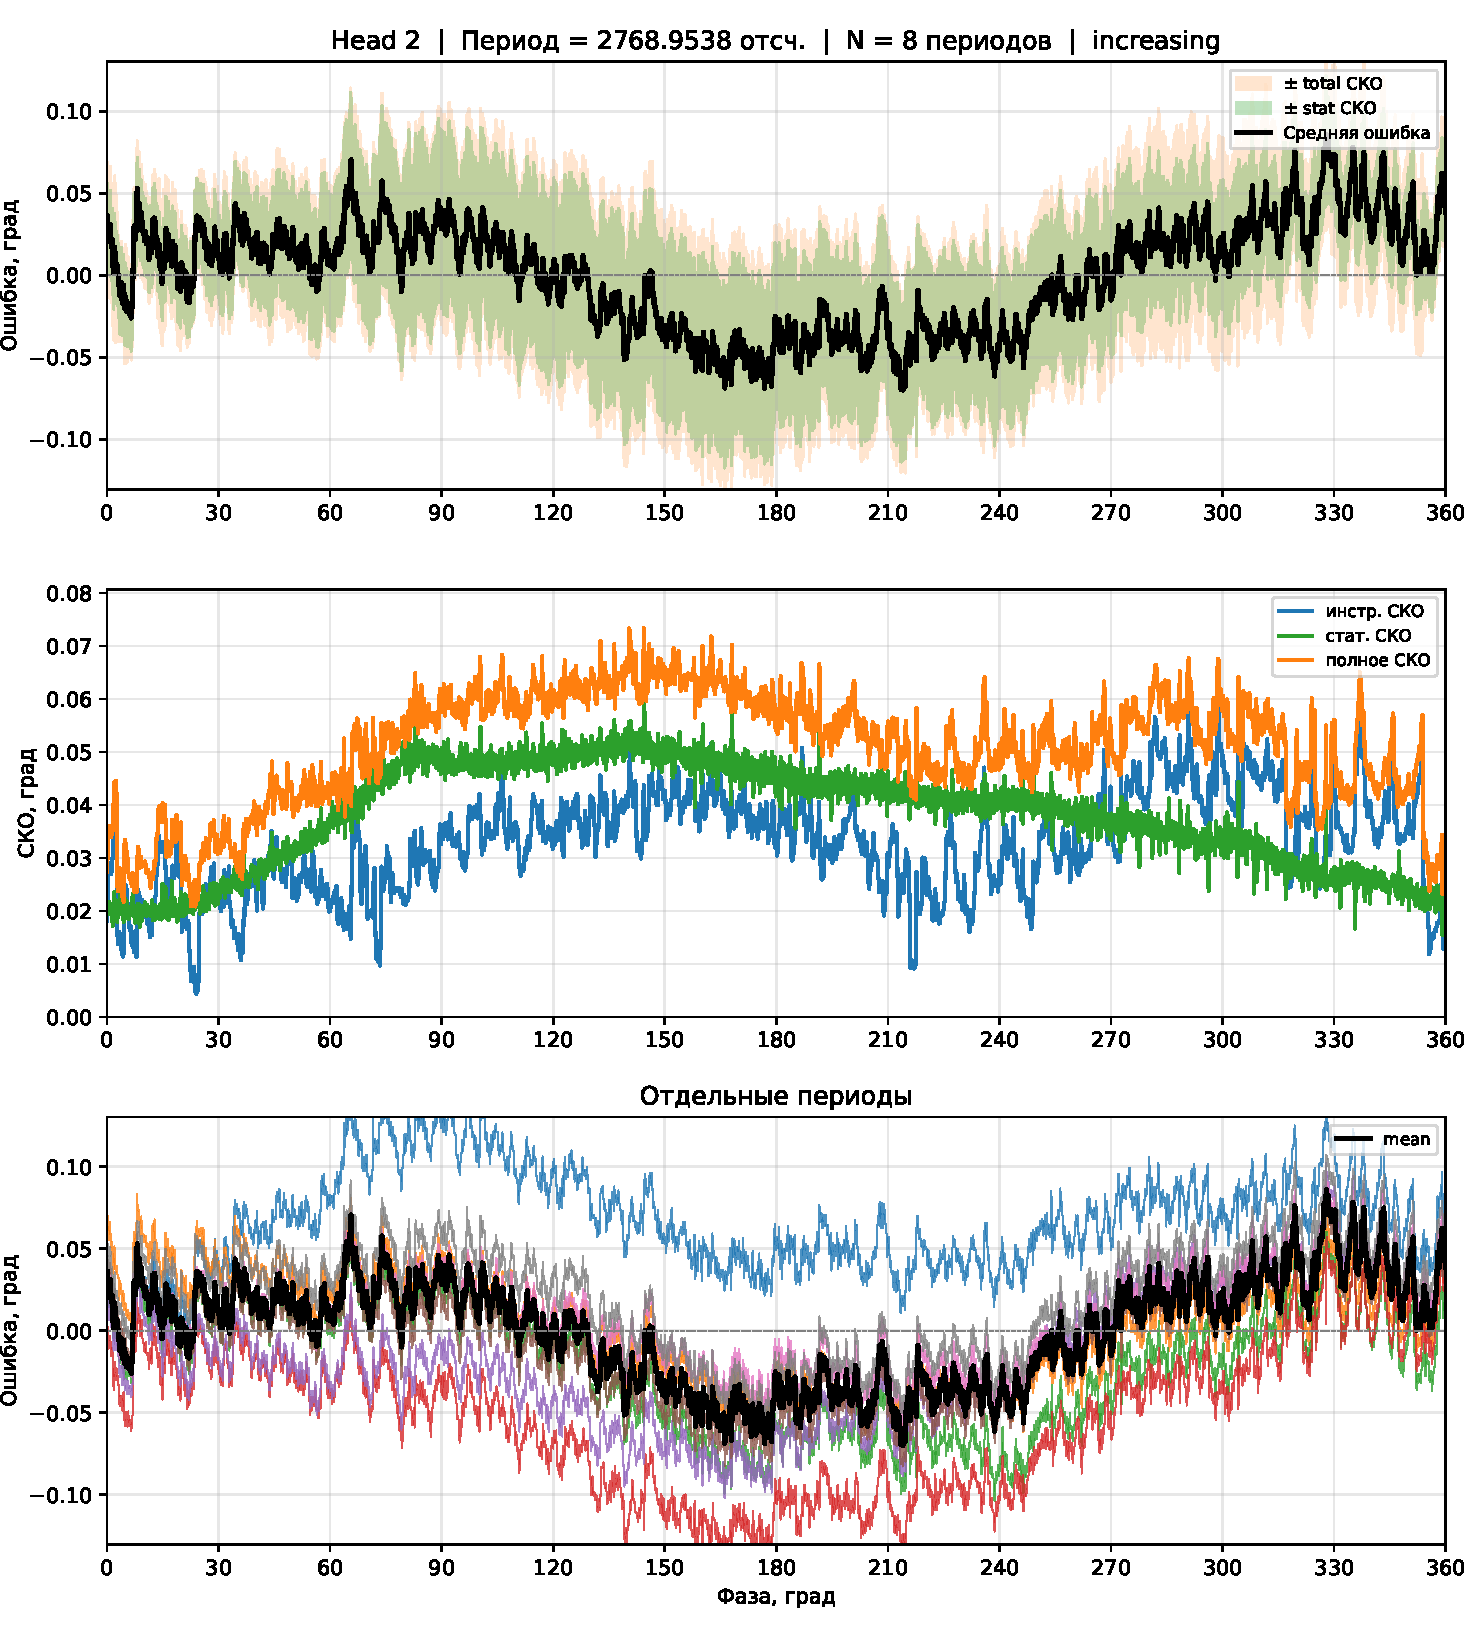
\includegraphics[width=\linewidth]{BespyatyyIV/images/final_10_5000_head2.pdf}
    \caption{Детрендированное усредненное по периодам показание второй головки при скорости 5000~микрошагов/с}
    \label{fig:head2}
\end{figure}
\newpage
\begin{figure}[ht!]
    \centering
    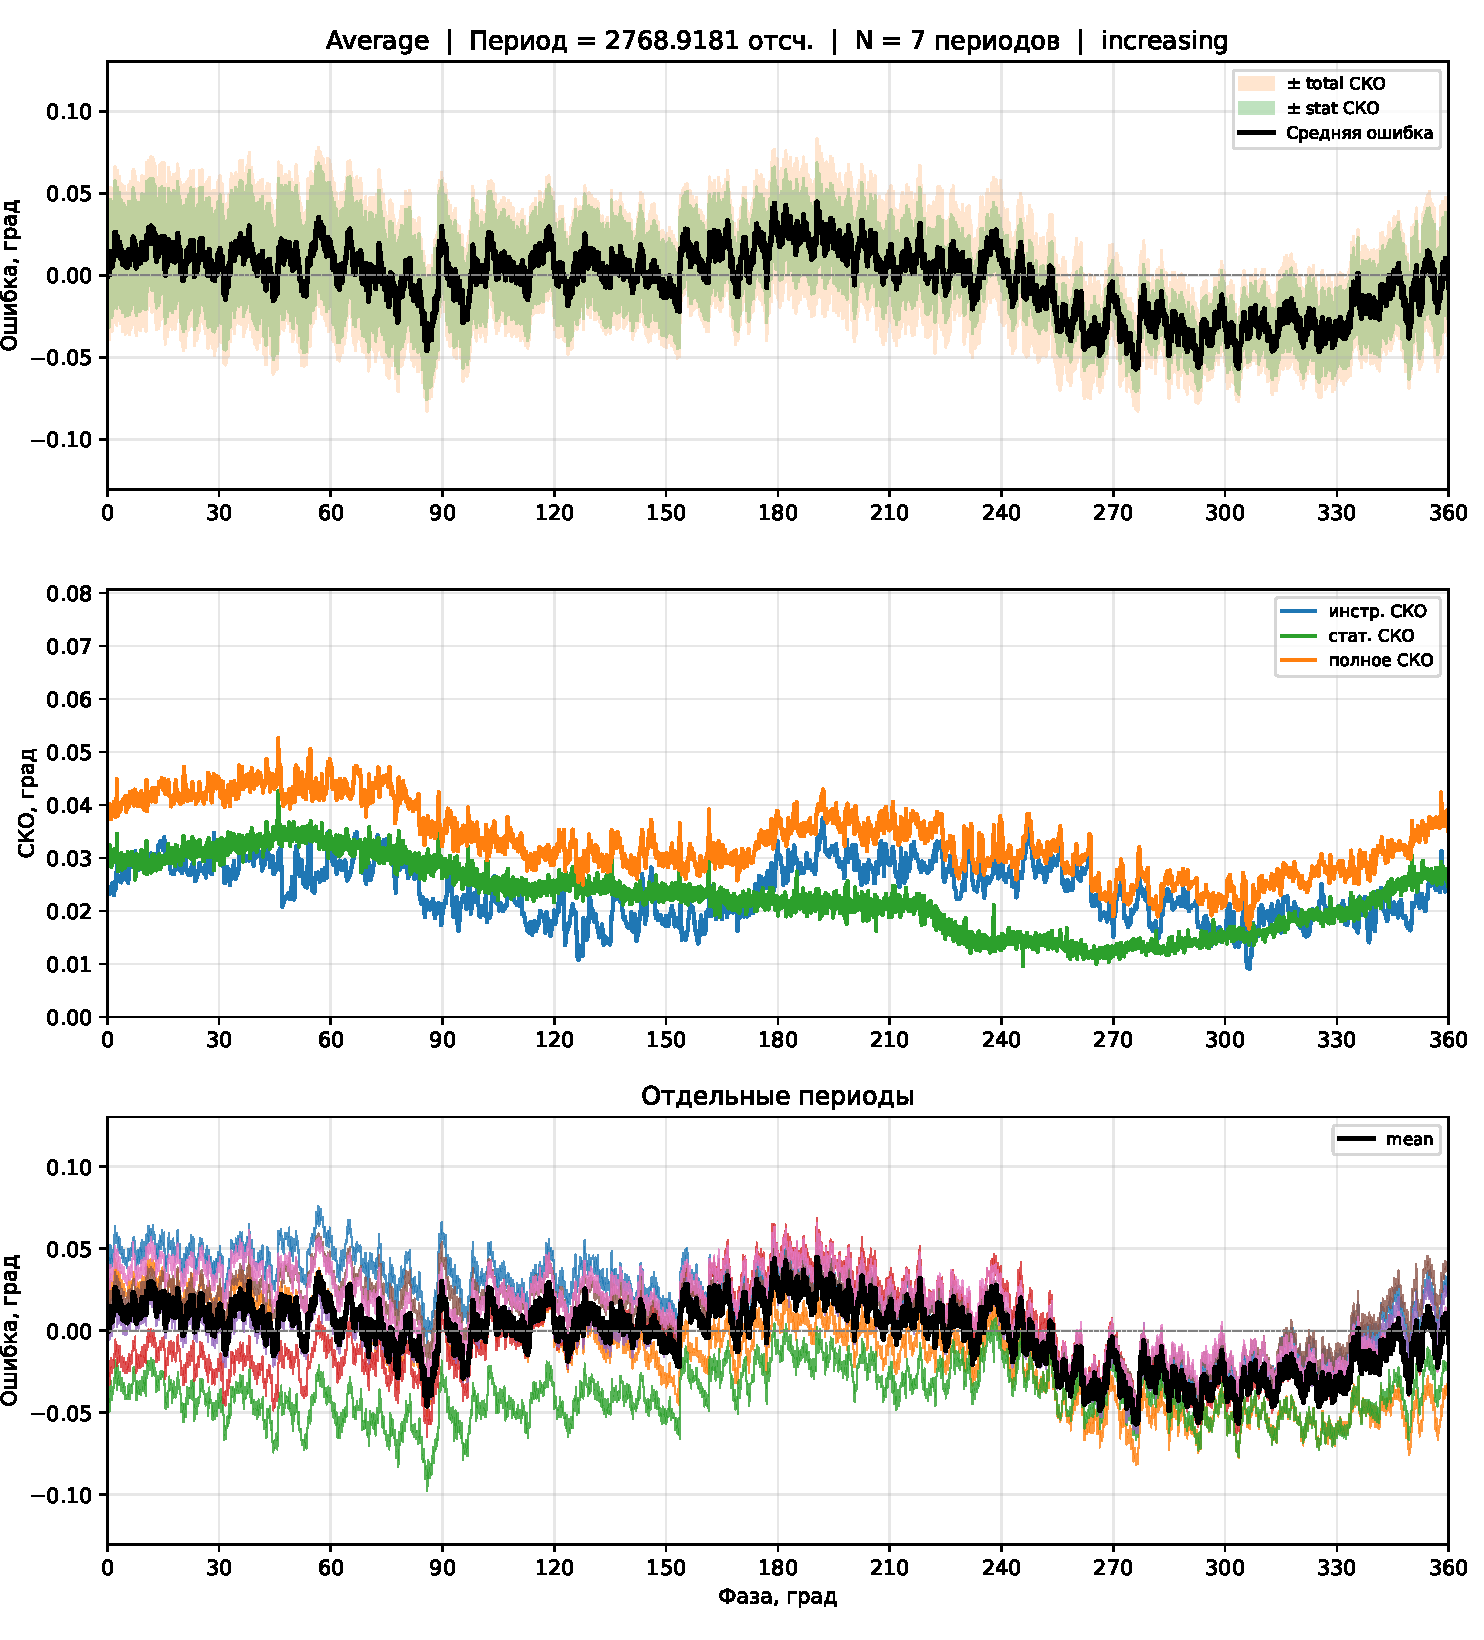
\includegraphics[width=\linewidth]{BespyatyyIV/images/final_10_5000_avg.pdf}
    \caption{Усредненная периодическая ошибка: круговое среднее двух головок при скорости 5000~микрошагов/с}
    \label{fig:avg}
\end{figure}
\newpage

%% ============================================================
%% СПИСОК ЛИТЕРАТУРЫ
%% ============================================================
\addcontentsline{toc}{section}{Список литературы}
\begin{thebibliography}{99}

\bibitem{renishaw_encoder_accuracy}
Renishaw.
The Accuracy of Rotary Encoders.
\url{https://www.renishaw.com/fr/the-accuracy-of-rotary-encoders--47130}.

\bibitem{eccentricity_error}
D.~Gurauskis, D.~Marinkovic, D.~Mažeika, A.~Kilikevičius.
Self-calibratable absolute modular rotary encoder:
development and experimental research.
\textit{Micromachines},
Vol.~15, No.~9, Art.~1130, 2024.
\url{https://doi.org/10.3390/mi15091130}.

\bibitem{heidenhain-modular-angle-encoders}
DR.~JOHANNES HEIDENHAIN GmbH.
Modular Angle Encoders with Circular Scale.
Technical brochure ID~1401414.
Traunreut, Germany.
\url{https://www.heidenhain.com/fileadmin/pdf/en/01_Products/Prospekte/PR_Modular_Angle_Encoders_Circular_Scale_ID1401414_en.pdf}.

\bibitem{mpu-ionak}
В.~Ф.~Ионак.
Приборы кинематического контроля.
М.: Машиностроение, 1981. 129~с.

\bibitem{mpu-bachish}
Е.~А.~Бачиш.
Методы воспроизведения единицы плоского угла.
\textit{Гироскопия и навигация},
№\,2, 2006, с.~105--112.

\bibitem{kiryanov-overview}
В.~П.~Кирьянов, А.~Д.~Петухов, А.~В.~Кирьянов.
Анализ алгоритмов самокалибровки в оптических датчиках угловых перемещений.
\textit{Автометрия},
Т.~58, №\,3, 2022, с.~12--23.
\url{https://doi.org/10.15372/AUT20220302}.

\bibitem{watanabe-eda}
T.~Watanabe, H.~Fujimoto, K.~Nakayama et al.
Automatic high-precision calibration system for angle encoder.
\textit{Proc.\ SPIE}, Vol.~4401, 2001, pp.~267--274.
\url{https://doi.org/10.1117/12.424900}.

\bibitem{singletrack_gray}
F.~Zhang, H.~Zhu, K.~Bian, P.~Liu, J.~Zhang.
Absolute position coding method for angular sensor --- single-track Gray codes.
\textit{Sensors (Basel)}, Vol.~18, No.~8, Art.~2728, 2018.
\url{https://doi.org/10.3390/s18082728}.

\bibitem{aleman_lens_distortion}
M.~Alemán-Flores, L.~Alvarez, L.~Gomez, D.~Santana-Cedrés.
Lens distortion models evaluation.
\textit{Image Processing On Line}, Vol.~4, 2014, pp.~183--200.
\url{https://doi.org/10.5201/ipol.2014.106}.

\bibitem{blais_rioux_peak}
F.~Blais, M.~Rioux.
Real-time numerical peak detector.
\textit{Signal Processing}, Vol.~11, No.~2, 1986, pp.~145--155.

\bibitem{TPoint_Wallace}
P.~T.~Wallace.
TPOINT --- Telescope Pointing Analysis System.
Starlink User Note 100.10, PPARC, 1994.
\url{https://sites.astro.caltech.edu/~srk/TP/Literature/Tpoint_SunWorks.pdf}.

\bibitem{Shatsky2020}
N.~Shatsky, A.~Belinski, A.~Dodin et al.
Caucasian Mountain Observatory of Sternberg Astronomical Institute:
First Six Years of Operation.
\textit{Proc.\ GBAR-2020}.
DOI:10.26119/978-5-6045062-0-2\_2020\_127.

\bibitem{EQMOD_Limits}
EQMOD Project.
Setting Limits on Equatorial Mount.
\url{https://eq-mod.sourceforge.net}.

\bibitem{habr_encoder}
Абсолютный поворотный энкодер с однодорожечным кодом Грея [Электронный ресурс] // Хабр, компания RUVDS.
02.12.2021.
URL: \url{https://habr.com/ru/companies/ruvds/articles/592201/}.

\bibitem{mostkom_patent}
А.~А.~Боев, С.~Н.~Кузнецов, А.~А.~Паршин, С.~Ю.~Поляков, С.~Е.~Широбакин.
Способ измерения угла поворота и устройство его реализующее.
Патент RU~2720052~C1, Опубликовано 23.04.2020.

\end{thebibliography}